\documentclass[12pt,a4paper]{article}

\usepackage[margin=1in]{geometry}
\usepackage{times}
\usepackage{graphicx}
\usepackage{setspace}
\usepackage{titlesec}
\usepackage{enumitem}
\usepackage{xurl}
\usepackage[hidelinks,breaklinks=true]{hyperref}
\usepackage{tikz}
\usepackage{eso-pic}
\usepackage{array}
\usepackage{booktabs}
\usepackage{listings}
\usepackage{xcolor}
\usepackage{float}
\usepackage{caption}
\usepackage[siunitx]{circuitikz}

\usetikzlibrary{shapes.geometric, arrows, positioning, calc, decorations.markings}

% Page border
\AddToShipoutPictureBG{%
  \begin{tikzpicture}[remember picture,overlay]
    \draw[thick]
      ([xshift=1cm,yshift=-1cm]current page.north west)
      rectangle
      ([xshift=-1cm,yshift=1cm]current page.south east);
  \end{tikzpicture}
}

\titleformat{\section}{\fontsize{16}{19.2}\bfseries\selectfont}{\thesection}{1em}{}
\titleformat{\subsection}{\fontsize{14}{16.8}\bfseries\selectfont}{\thesubsection}{1em}{}
\titleformat{\subsubsection}{\fontsize{12}{14.4}\bfseries\selectfont}{\thesubsubsection}{1em}{}

% Code listing style
\definecolor{codebg}{RGB}{245,245,245}
\definecolor{codegreen}{RGB}{0,128,0}
\definecolor{codeblue}{RGB}{0,0,180}
\definecolor{codegray}{RGB}{128,128,128}
\definecolor{codepurple}{RGB}{128,0,128}

\lstdefinestyle{arduinoStyle}{
    backgroundcolor=\color{codebg},
    commentstyle=\color{codegreen}\itshape,
    keywordstyle=\color{codeblue}\bfseries,
    stringstyle=\color{codepurple},
    basicstyle=\ttfamily\footnotesize,
    breakatwhitespace=false,
    breaklines=true,
    captionpos=b,
    keepspaces=true,
    numbers=left,
    numbersep=8pt,
    numberstyle=\tiny\color{codegray},
    showspaces=false,
    showstringspaces=false,
    showtabs=false,
    tabsize=2,
    frame=single,
    rulecolor=\color{codegray},
    framesep=5pt,
    xleftmargin=15pt,
    language=C++,
    morekeywords={String, Serial, pinMode, analogWrite, OUTPUT, LOW, HIGH, setup, loop, void, int, char, const, delay},
}

\begin{document}

% ===== TITLE PAGE =====
\begin{center}
    \includegraphics[width=3cm]{"Bangalore_University_logo1.png"}\\[0.5cm]
    {\fontsize{18}{21.6}\bfseries BENGALURU UNIVERSITY}\\[0.5cm]
    {\fontsize{14}{16.8}\selectfont Jnana Bharathi campus Bengaluru-560001}\\[1cm]
    
    \includegraphics[width=3cm]{"shree daksha academy.png"}\\[0.5cm]
    {\fontsize{18}{21.6}\bfseries SHREE DAKSHA ACADEMY}\\[0.5cm]
    {\fontsize{16}{19.2}\bfseries DEPARTMENT OF COMPUTER SCIENCE}\\[1.5cm]
    
    {\fontsize{16}{19.2}\selectfont `` \textit{SmartBreeze: Hardware Technical Documentation} ''}\\[1cm]

\end{center}
\vspace{1cm}
\begin{minipage}{0.45\textwidth}
    \begin{flushleft}
        \fontsize{14}{16.8}\selectfont
        \underline{\bfseries SUBMITTED TO}\\[0.5cm]
        \fontsize{12}{14.4}\selectfont
        \textbf{CHAITRA SR}\\
        (Dept of CS)
    \end{flushleft}
\end{minipage}
\hfill
\begin{minipage}{0.45\textwidth}
    \begin{flushright}
        \fontsize{14}{16.8}\selectfont
        \underline{\bfseries SUBMITTED BY}\\[0.5cm]
        \fontsize{12}{14.4}\selectfont
        \textbf{YOGESH MN}\\
        (U03HC23S0055)
    \end{flushright}
\end{minipage}

\vspace{3cm}

\newpage

\onehalfspacing

% ===== TABLE OF CONTENTS =====
\tableofcontents
\newpage

% ===== SECTION 1: INTRODUCTION =====
\section{Introduction}
This document serves as the complete hardware technical reference for the \textbf{SmartBreeze} project. It details the electronic circuit design, individual component specifications, wiring connections, the Arduino microcontroller firmware, and the browser-based communication protocol used to bridge the web application with the physical fan hardware.

The system uses a \textbf{WebUSB/Web Serial API} to transmit real-time PWM (Pulse Width Modulation) speed values from a web browser directly to an Arduino Nano microcontroller, which in turn drives a 12V DC brushless fan through a transistor switching circuit.

% ===== SECTION 2: COMPONENTS =====
\section{Hardware Components}

\subsection{Bill of Materials}

\begin{table}[H]
\centering
\renewcommand{\arraystretch}{1.4}
\begin{tabular}{|>{\raggedright}p{0.6cm}|>{\raggedright}p{4.2cm}|>{\raggedright}p{3.5cm}|>{\raggedright}p{2cm}|>{\raggedright\arraybackslash}p{3.5cm}|}
\hline
\textbf{S.N.} & \textbf{Component} & \textbf{Specification} & \textbf{Qty} & \textbf{Purpose} \\
\hline
1 & Arduino Nano & ATmega328P, 5V, 16MHz & 1 & Microcontroller (PWM generation) \\
\hline
2 & 12V DC Brushless Fan & 12V, 0.15A--0.30A & 1 & Actuator (cooling fan) \\
\hline
3 & TIP120 Darlington Transistor & NPN, 60V, 5A & 1 & High-current switching element \\
\hline
4 & 1N4007 Flyback Diode & 1000V, 1A & 1 & Reverse EMF protection \\
\hline
5 & 1K$\Omega$ Resistor & 1/4W, Carbon Film & 1 & Base current limiter \\
\hline
6 & 12V DC Power Adapter & 12V, 1A output & 1 & External fan power supply \\
\hline
7 & Breadboard & 830 tie-points, full-size & 1 & Prototyping platform \\
\hline
8 & Jumper Wires & Male-to-Male & 7--8 & Inter-component connections \\
\hline
9 & USB Cable & USB Mini-B / USB-C & 1 & Arduino to PC/Phone link \\
\hline
10 & USB OTG Adapter & USB-C to USB-A & 1 & Mobile phone connectivity \\
\hline
11 & DC Female Power Jack & 5.5mm x 2.1mm barrel & 1 & 12V adapter socket on breadboard \\
\hline
\end{tabular}
\caption{Complete Bill of Materials for the SmartBreeze Circuit}
\label{tab:bom}
\end{table}

\newpage

\subsection{Component Descriptions}

\subsubsection{Arduino Nano (ATmega328P)}
\begin{minipage}[t]{0.62\textwidth}
\vspace{0pt}
The Arduino Nano is a compact, breadboard-friendly microcontroller board based on the ATmega328P chip. It features 14 digital I/O pins (6 of which provide PWM output), 8 analog inputs, a 16 MHz ceramic resonator, and USB connectivity. In this project, \textbf{Pin D9} is configured as the PWM output channel to generate variable-duty-cycle signals for fan speed control.
\end{minipage}
\hfill
\begin{minipage}[t]{0.33\textwidth}
\vspace{0pt}
\centering
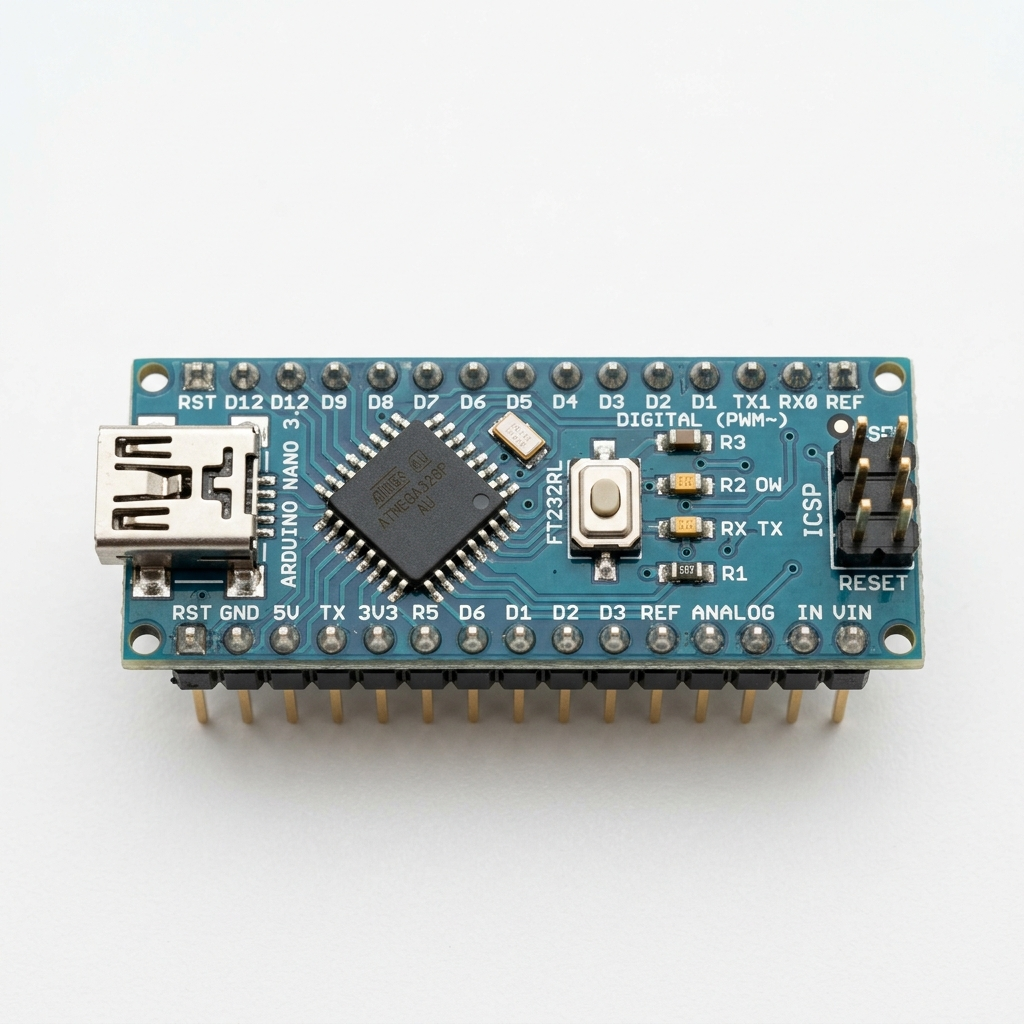
\includegraphics[width=\textwidth]{images/arduino_nano.png}
\captionof{figure}{Arduino Nano}
\end{minipage}

\vspace{0.8cm}

\subsubsection{TIP120 Darlington Transistor}
\begin{minipage}[t]{0.62\textwidth}
\vspace{0pt}
The TIP120 is an NPN Darlington pair transistor capable of switching currents up to 5A. Since the Arduino's digital pins can only source approximately 20mA, the TIP120 acts as a \textbf{power amplifier} --- a small signal from Pin D9 controls the much larger 12V current flowing through the fan motor. The Darlington configuration provides a current gain ($h_{FE}$) of approximately 1000, making it ideal for this application.
\end{minipage}
\hfill
\begin{minipage}[t]{0.33\textwidth}
\vspace{0pt}
\centering
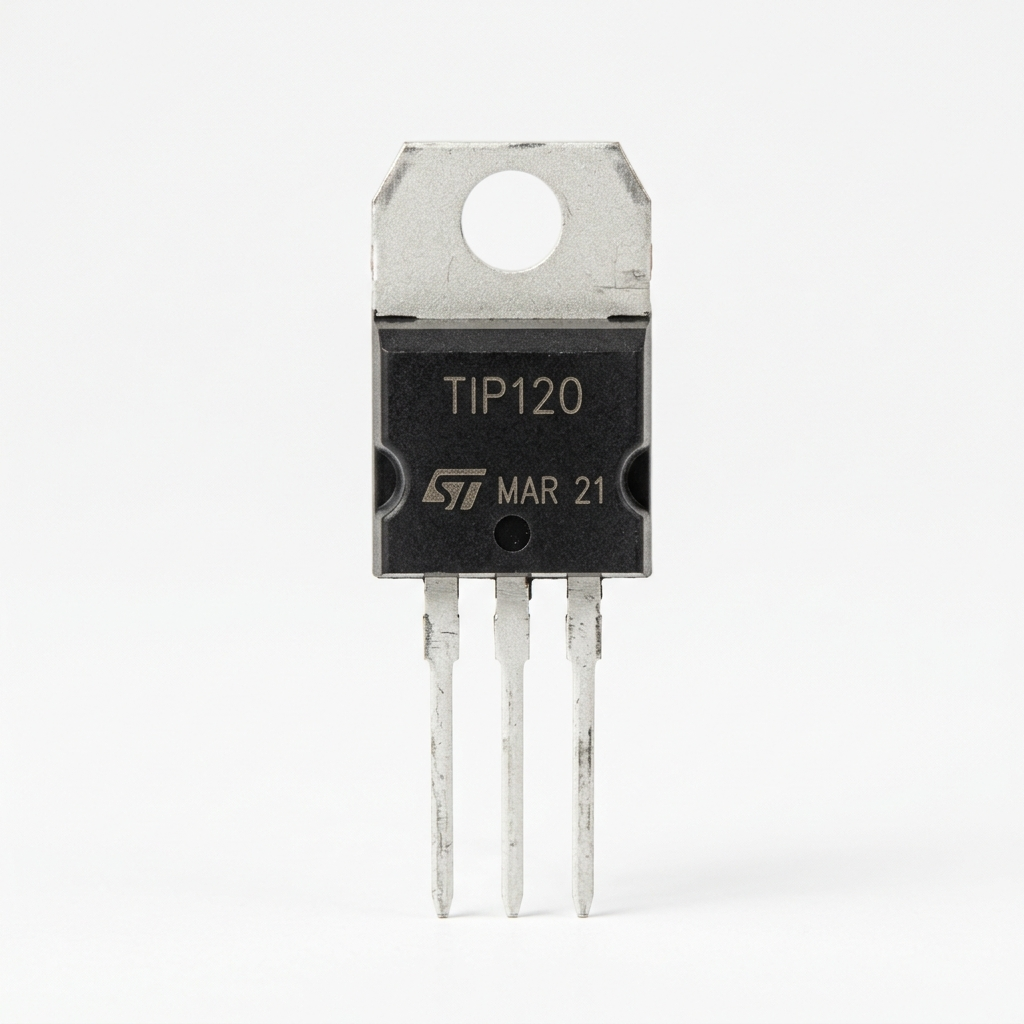
\includegraphics[width=\textwidth]{images/tip120_transistor.png}
\captionof{figure}{TIP120 Transistor}
\end{minipage}

\vspace{0.8cm}

\subsubsection{1N4007 Flyback Protection Diode}
\begin{minipage}[t]{0.62\textwidth}
\vspace{0pt}
DC motors generate a reverse voltage spike (back-EMF) when they are switched off or when their speed changes rapidly. The 1N4007 diode is placed \textbf{in reverse-bias across the fan terminals} to safely absorb these voltage spikes, protecting the TIP120 transistor and the Arduino from damage.
\end{minipage}
\hfill
\begin{minipage}[t]{0.33\textwidth}
\vspace{0pt}
\centering
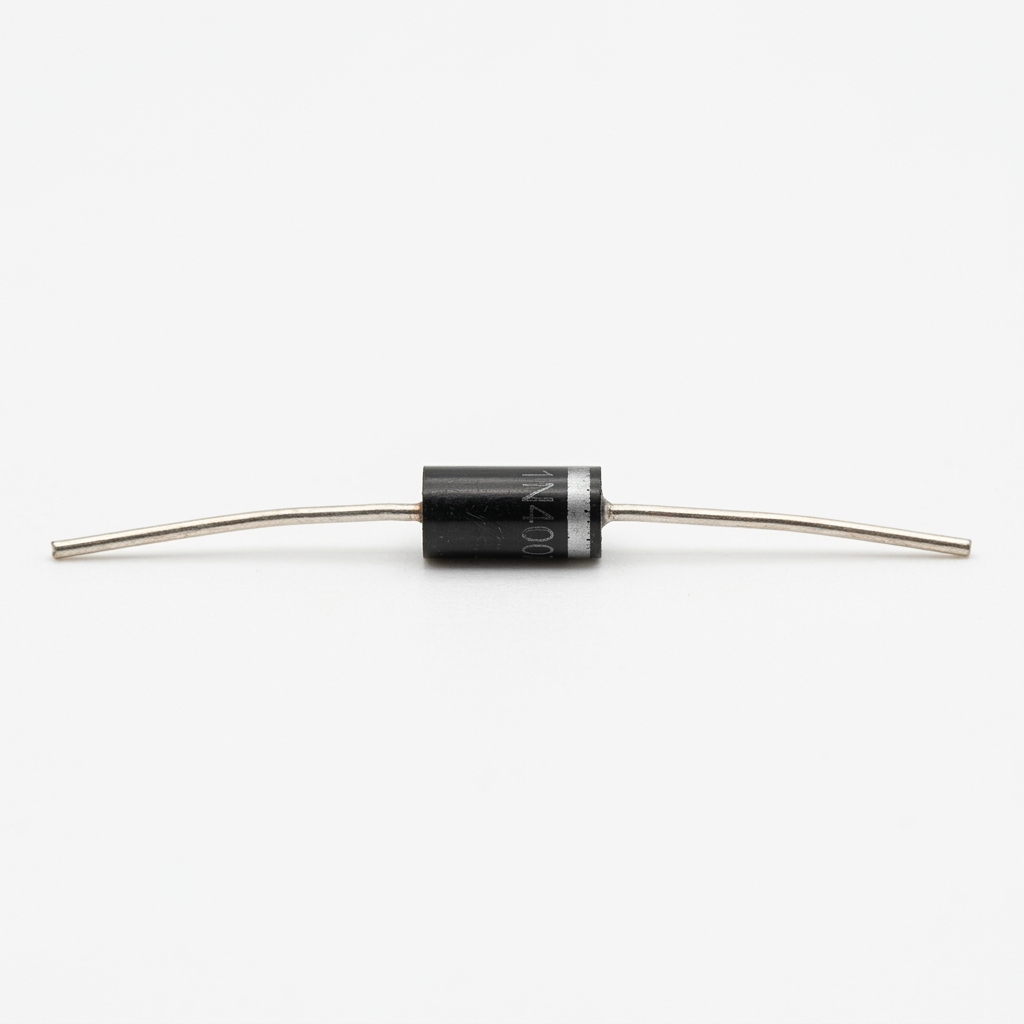
\includegraphics[width=\textwidth]{images/diode_1n4007.png}
\captionof{figure}{1N4007 Diode}
\end{minipage}

\vspace{0.8cm}

\subsubsection{1K$\Omega$ Base Resistor}
\begin{minipage}[t]{0.62\textwidth}
\vspace{0pt}
This resistor limits the current flowing from Arduino Pin D9 into the Base pin of the TIP120 transistor. Without this resistor, excessive current could damage the Arduino's GPIO pin. The value is calculated as:
\[
R_{base} = \frac{V_{pin} - V_{BE}}{I_{base}} = \frac{5V - 1.4V}{3.6mA} \approx 1K\Omega
\]
where $V_{BE}$ is the Darlington pair's base-emitter voltage drop (approximately 1.4V).
\end{minipage}
\hfill
\begin{minipage}[t]{0.33\textwidth}
\vspace{0pt}
\centering
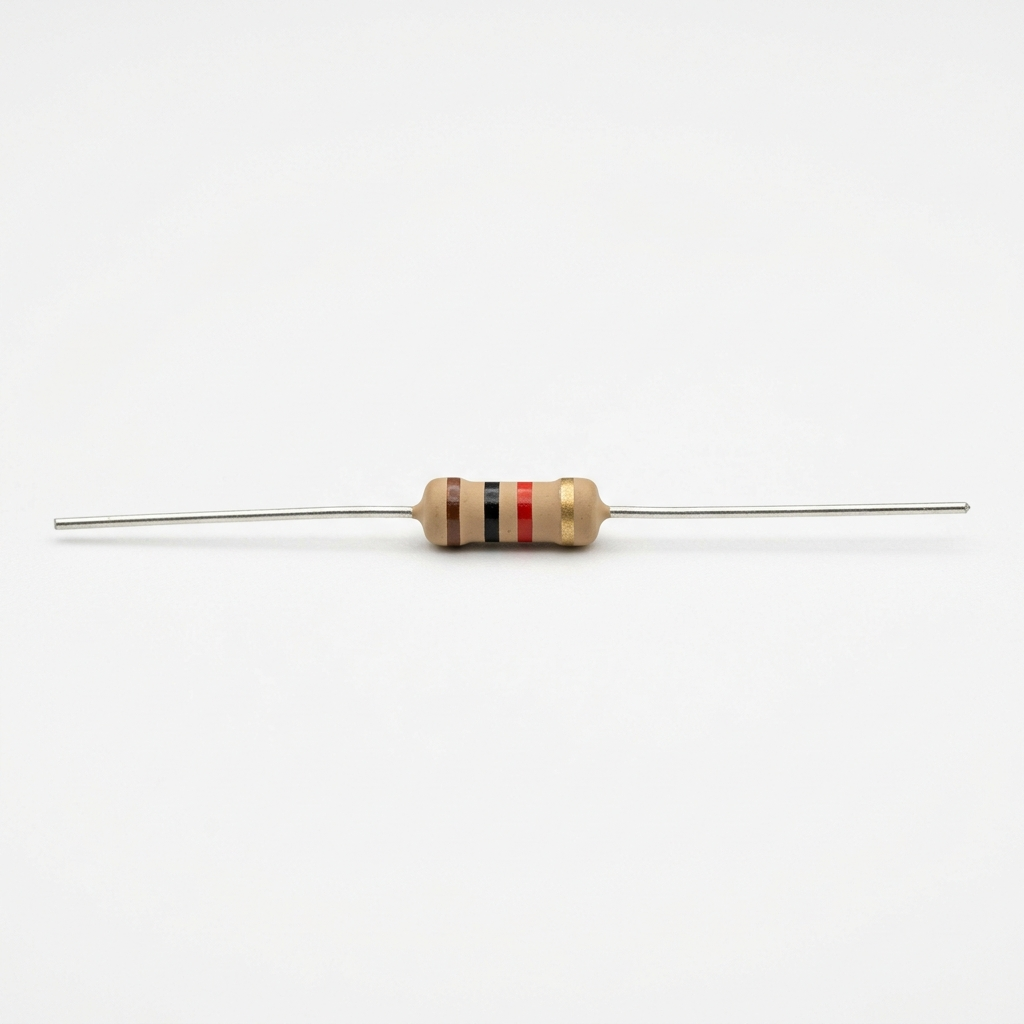
\includegraphics[width=\textwidth]{images/resistor_1k.png}
\captionof{figure}{1K$\Omega$ Resistor}
\end{minipage}

\vspace{0.8cm}

\subsubsection{12V DC Brushless Fan}
\begin{minipage}[t]{0.62\textwidth}
\vspace{0pt}
The 12V DC brushless cooling fan is the primary actuator of the system. It converts electrical energy into mechanical airflow. The fan's speed is proportional to the average voltage applied across its terminals, which is controlled via PWM switching through the TIP120 transistor. Typical current draw ranges from 0.15A to 0.30A.
\end{minipage}
\hfill
\begin{minipage}[t]{0.33\textwidth}
\vspace{0pt}
\centering
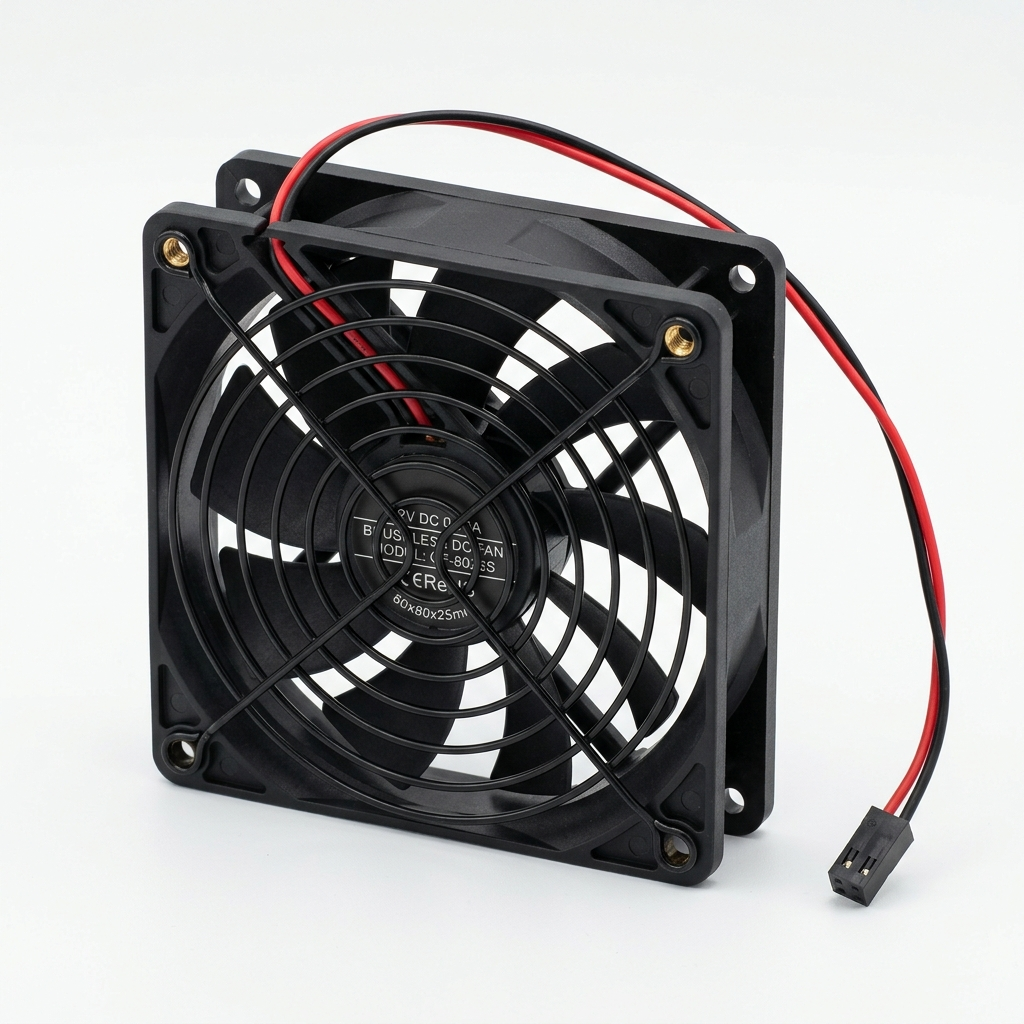
\includegraphics[width=\textwidth]{images/dc_fan_12v.png}
\captionof{figure}{12V DC Fan}
\end{minipage}

\vspace{0.8cm}

\subsubsection{12V DC Power Adapter}
\begin{minipage}[t]{0.62\textwidth}
\vspace{0pt}
The external 12V adapter provides the high-voltage power required by the fan motor. The Arduino's 5V rail is insufficient to drive a 12V motor, hence a separate power source is necessary. The adapter's ground must be shared with the Arduino's ground to complete the circuit. Rated output: 12V, 1A DC.
\end{minipage}
\hfill
\begin{minipage}[t]{0.33\textwidth}
\vspace{0pt}
\centering
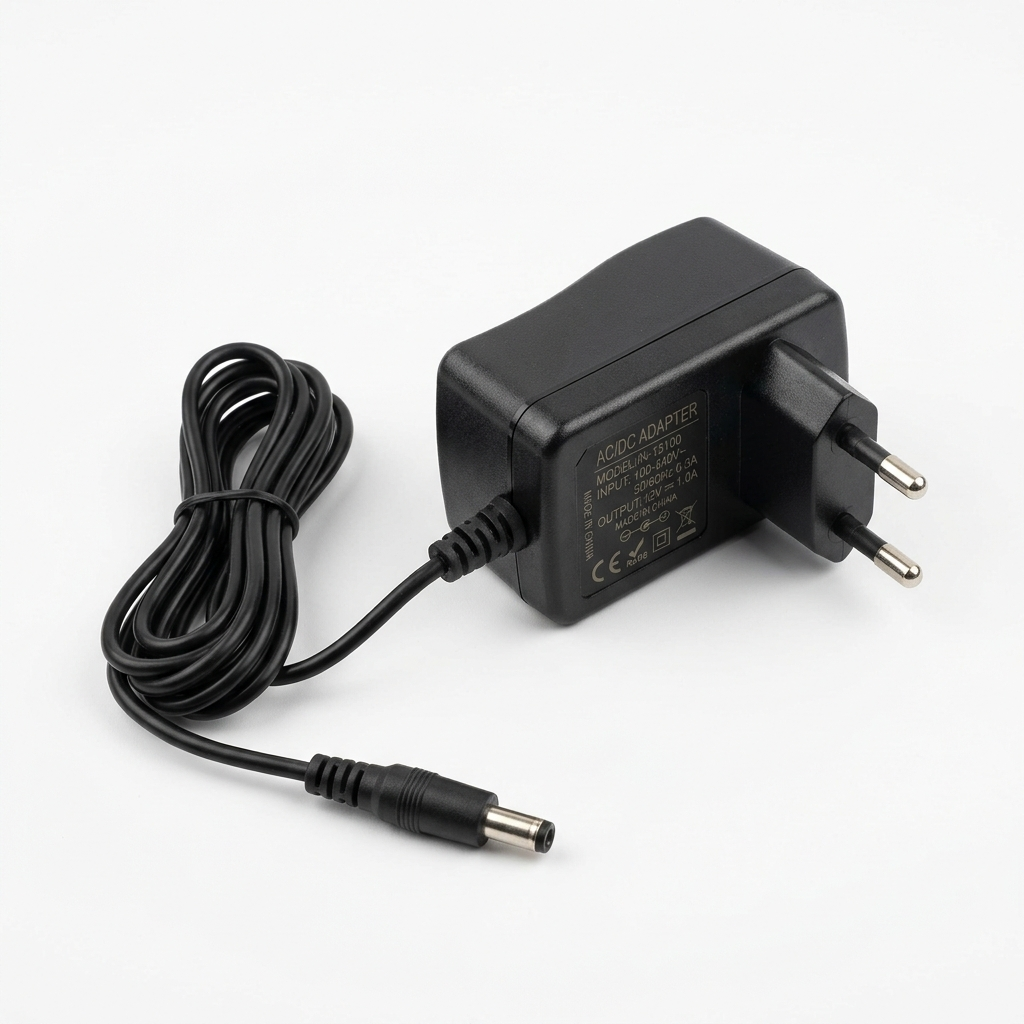
\includegraphics[width=\textwidth]{images/power_adapter_12v.png}
\captionof{figure}{12V DC Adapter}
\end{minipage}

\newpage

\subsection{Supporting Components}

\noindent
\begin{minipage}[t]{0.30\textwidth}
\centering
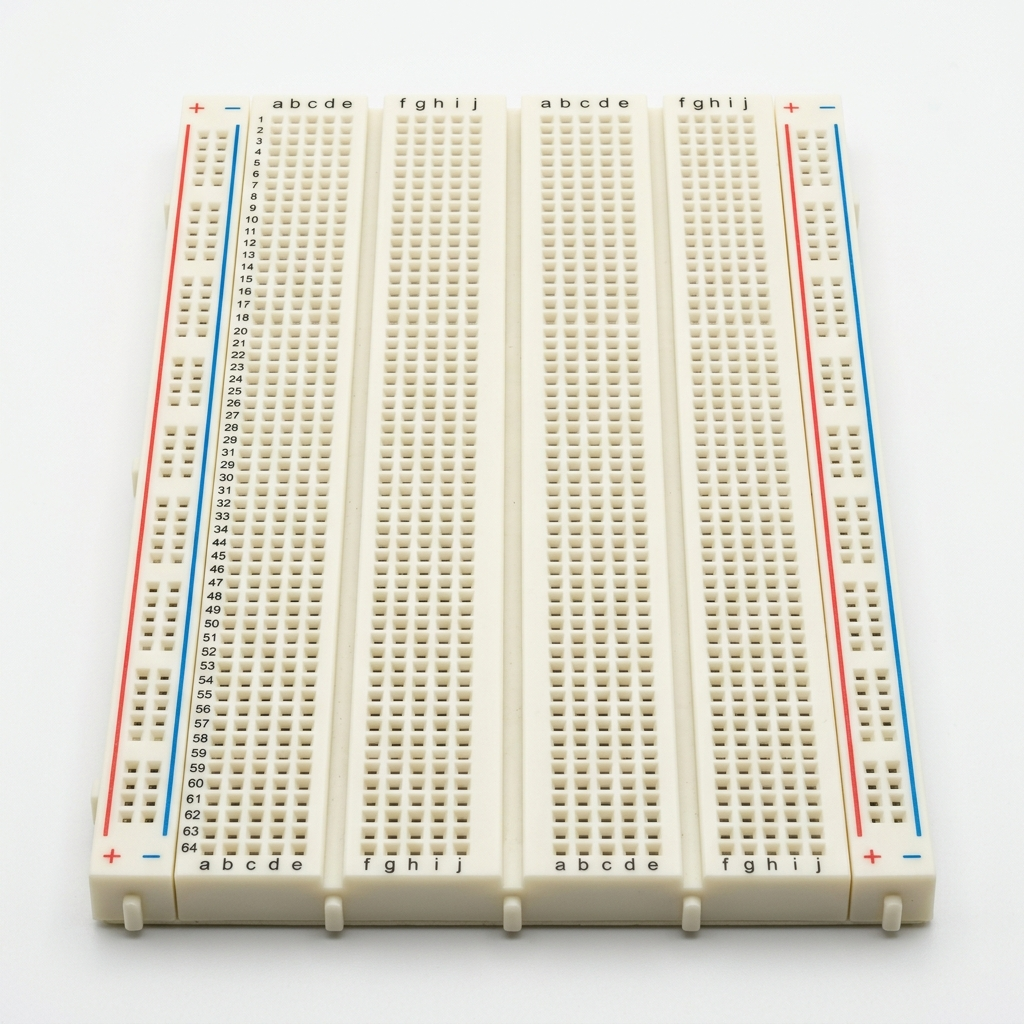
\includegraphics[width=\textwidth]{images/breadboard.png}
\captionof{figure}{830-Point Breadboard}
\end{minipage}
\hfill
\begin{minipage}[t]{0.30\textwidth}
\centering
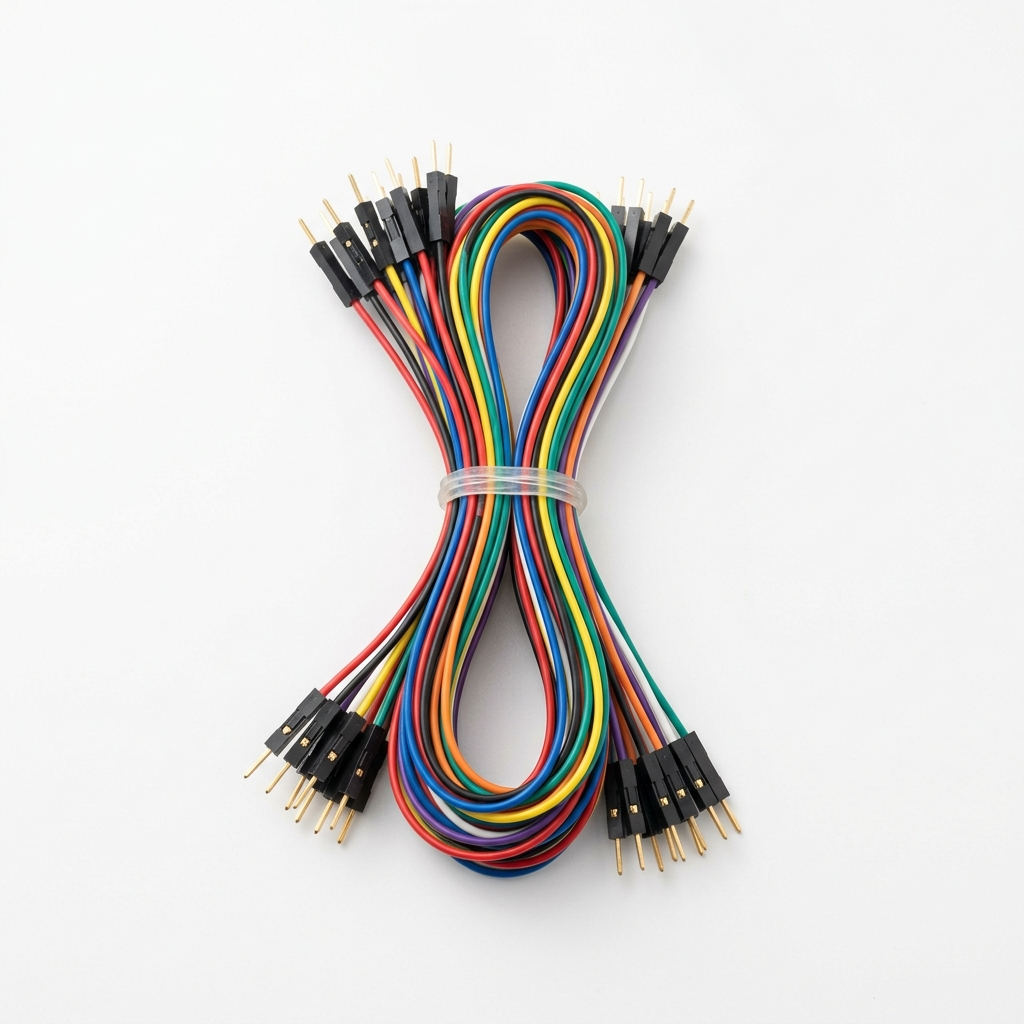
\includegraphics[width=\textwidth]{images/jumper_wires.png}
\captionof{figure}{Jumper Wires (M-to-M)}
\end{minipage}
\hfill
\begin{minipage}[t]{0.30\textwidth}
\centering
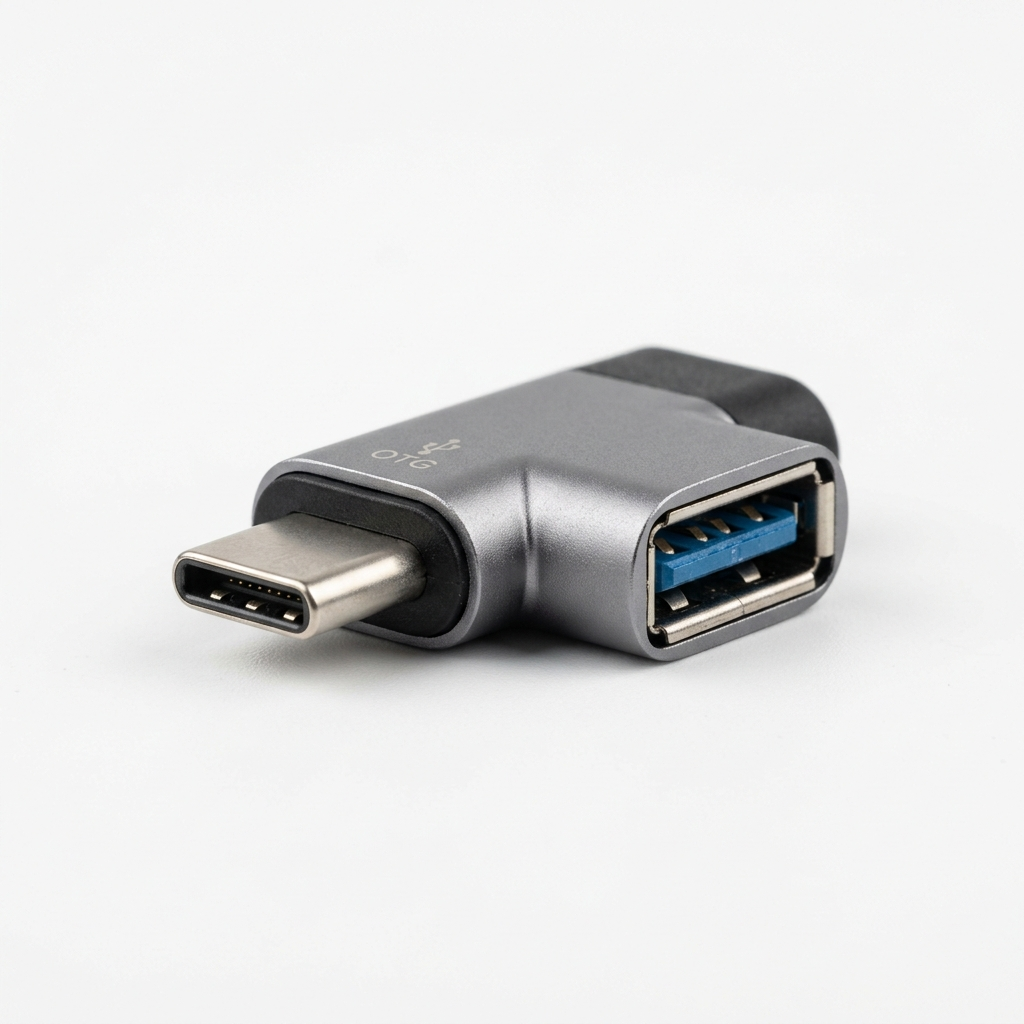
\includegraphics[width=\textwidth]{images/usb_otg_adapter.png}
\captionof{figure}{USB-C OTG Adapter}
\end{minipage}

\vspace{1cm}

\noindent
\begin{minipage}[t]{0.30\textwidth}
\centering
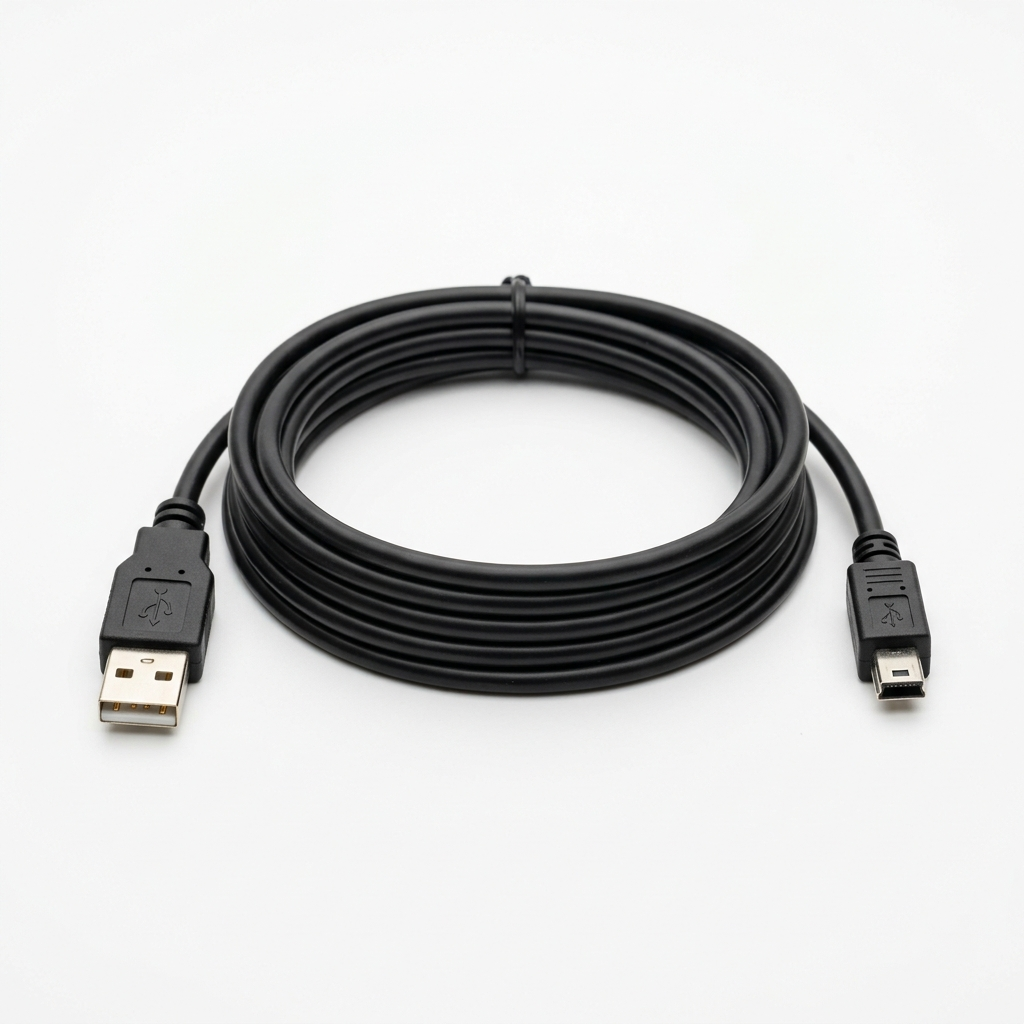
\includegraphics[width=\textwidth]{images/usb_cable.png}
\captionof{figure}{USB Mini-B Cable}
\end{minipage}
\hfill
\begin{minipage}[t]{0.30\textwidth}
\centering
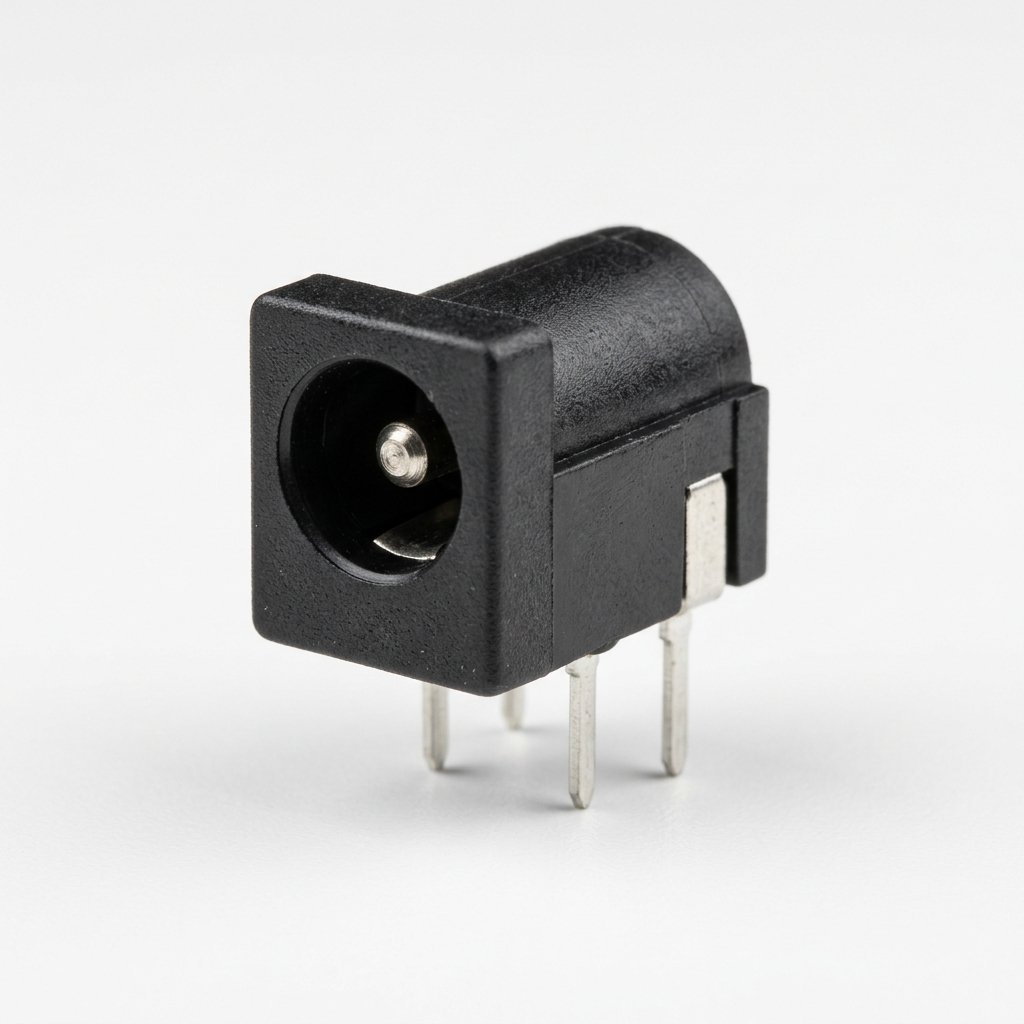
\includegraphics[width=\textwidth]{images/dc_power_jack.png}
\captionof{figure}{DC Female Power Jack}
\end{minipage}
\hfill
\begin{minipage}[t]{0.30\textwidth}
\hfill
\end{minipage}

\vspace{0.5cm}

\begin{itemize}
    \item \textbf{Breadboard (830 tie-points):} A solderless prototyping platform used to assemble the circuit without permanent soldering. Components are inserted into the grid of holes and connected via internal metal clips.
    \item \textbf{Jumper Wires (Male-to-Male):} Flexible wires with pin headers used to create electrical connections between the breadboard rows and the Arduino's header pins.
    \item \textbf{USB OTG Adapter (USB-C to USB-A):} Enables direct connection between an Android smartphone and the Arduino Nano, allowing the mobile web application to communicate with the hardware via WebUSB.
    \item \textbf{USB Mini-B Cable:} Connects the Arduino Nano to the PC or laptop. Carries both power (5V from USB) and serial data for firmware upload and real-time communication with the web application.
    \item \textbf{DC Female Power Jack:} A barrel socket connector mounted on the breadboard that accepts the 12V DC adapter plug. Provides a secure, detachable connection point for the external fan power supply, with positive and negative terminals routed to the breadboard's power rails.
\end{itemize}

\newpage



% ===== SECTION 3: CIRCUIT DIAGRAM =====
\section{Circuit Diagram}

\subsection{Schematic Diagram}

\begin{figure}[H]
\centering
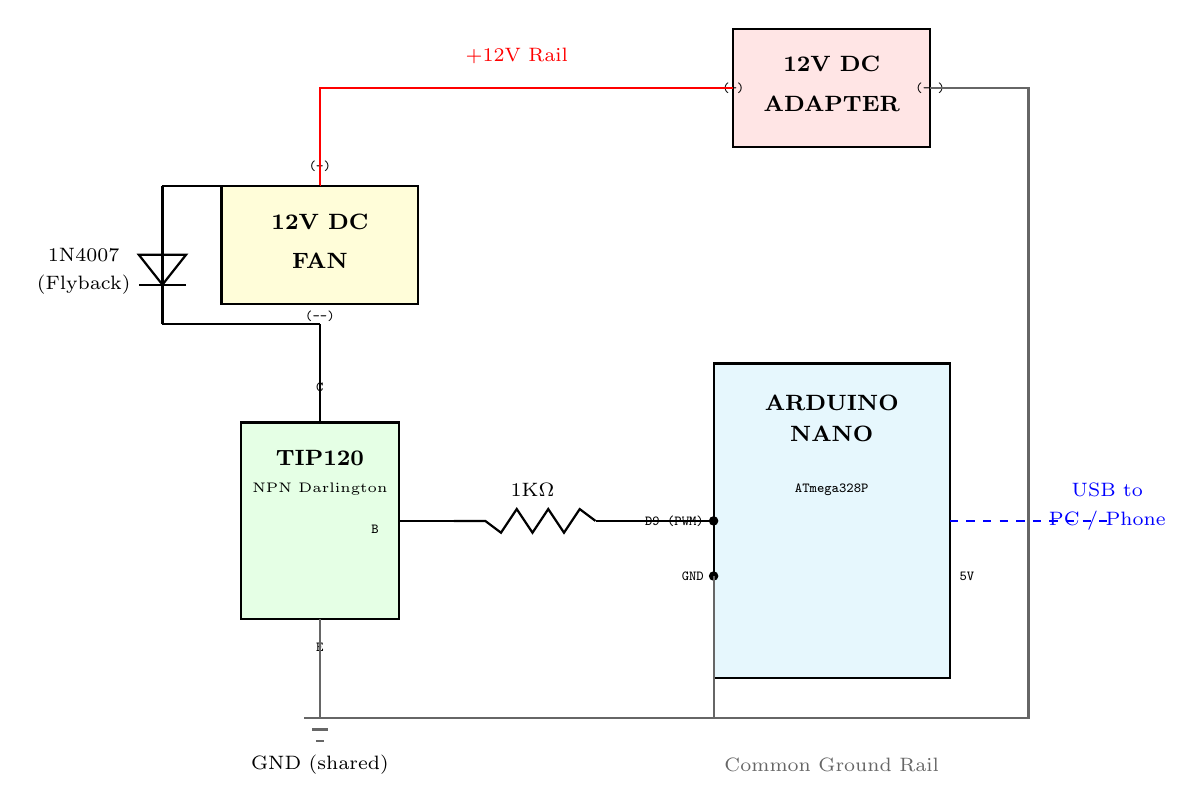
\begin{tikzpicture}[scale=1.0, transform shape,
    component/.style={draw, thick, rectangle, minimum width=2.2cm, minimum height=1.2cm, fill=blue!8, font=\footnotesize\bfseries},
    pin/.style={font=\tiny\ttfamily},
    wire/.style={thick, draw=black},
    pwire/.style={thick, draw=red},
    gwire/.style={thick, draw=black!60},
    label/.style={font=\scriptsize}
]

% Arduino Nano
\node[component, minimum width=3cm, minimum height=4cm, fill=cyan!10] (arduino) at (0,0) {};
\node[font=\footnotesize\bfseries] at (0,1.5) {ARDUINO};
\node[font=\footnotesize\bfseries] at (0,1.1) {NANO};
\node[pin] at (0,0.4) {ATmega328P};

% Arduino pins
\node[pin, anchor=east] (d9) at (-1.5,0) {D9 (PWM)};
\node[pin, anchor=east] (gnd) at (-1.5,-0.7) {GND};
\node[pin, anchor=west] (vin) at (1.5,-0.7) {5V};
\draw[fill=black] (-1.5,0) circle (1.5pt);
\draw[fill=black] (-1.5,-0.7) circle (1.5pt);

% Resistor
\node[label] at (-3.8,0.4) {1K$\Omega$};
\draw[wire] (-1.5,0) -- (-3,0);
\draw[thick] (-3,0) -- (-3.2,0.15) -- (-3.4,-0.15) -- (-3.6,0.15) -- (-3.8,-0.15) -- (-4,0.15) -- (-4.2,-0.15) -- (-4.4,0) -- (-4.8,0);

% TIP120 Transistor
\node[component, minimum width=2cm, minimum height=2.5cm, fill=green!10] (tip) at (-6.5,0) {};
\node[font=\footnotesize\bfseries] at (-6.5,0.8) {TIP120};
\node[font=\tiny] at (-6.5,0.4) {NPN Darlington};

% TIP120 pins
\node[pin] at (-5.8,-0.1) {B};
\node[pin] at (-6.5,-1.6) {E};
\node[pin] at (-6.5,1.7) {C};

% Base connection
\draw[wire] (-4.8,0) -- (-5.5,0) -- (-5.5,-0.1);

% Emitter to ground
\draw[gwire] (-6.5,-1.25) -- (-6.5,-2.5);
\draw[gwire] (-6.7,-2.5) -- (-6.3,-2.5);
\draw[gwire] (-6.6,-2.65) -- (-6.4,-2.65);
\draw[gwire] (-6.55,-2.8) -- (-6.45,-2.8);
\node[label] at (-6.5,-3.1) {GND (shared)};

% Common ground connection from Arduino
\draw[gwire] (-1.5,-0.7) -- (-1.5,-2.5) -- (-6.5,-2.5);

% Collector to Fan
\draw[wire] (-6.5,1.25) -- (-6.5,2.5);

% 12V DC Fan
\node[component, minimum width=2.5cm, minimum height=1.5cm, fill=yellow!15] (fan) at (-6.5,3.5) {};
\node[font=\footnotesize\bfseries] at (-6.5,3.8) {12V DC};
\node[font=\footnotesize\bfseries] at (-6.5,3.3) {FAN};
\node[pin] at (-6.5,2.6) {(--)};
\node[pin] at (-6.5,4.5) {(+)};

% Fan to 12V supply
\draw[pwire] (-6.5,4.25) -- (-6.5,5.5) -- (-2,5.5);

% 12V Power Supply
\node[component, minimum width=2.5cm, minimum height=1.5cm, fill=red!10] (psu) at (0,5.5) {};
\node[font=\footnotesize\bfseries] at (0,5.8) {12V DC};
\node[font=\footnotesize\bfseries] at (0,5.3) {ADAPTER};
\node[pin] at (-1.25,5.5) {(+)};
\node[pin] at (1.25,5.5) {(--)};

% Power supply positive to fan
\draw[pwire] (-1.25,5.5) -- (-2,5.5);

% Power supply ground
\draw[gwire] (1.25,5.5) -- (2.5,5.5) -- (2.5,-2.5) -- (-1.5,-2.5);

% Flyback Diode across fan
\draw[wire] (-8.5,2.5) -- (-8.5,4.25);
\draw[wire] (-6.5,2.5) -- (-8.5,2.5);
\draw[wire] (-6.5,4.25) -- (-8.5,4.25);

% Diode symbol
\draw[thick] (-8.5,3.0) -- (-8.2,3.38) -- (-8.8,3.38) -- cycle;
\draw[thick] (-8.2,3.0) -- (-8.8,3.0);
\node[label] at (-9.5,3.38) {1N4007};
\node[label] at (-9.5,3.0) {(Flyback)};

% USB connection indicator
\draw[thick, blue, dashed] (1.5,0) -- (3.5,0);
\node[font=\scriptsize\color{blue}] at (3.5,0.4) {USB to};
\node[font=\scriptsize\color{blue}] at (3.5,0) {PC / Phone};

% Labels for voltage rails
\node[font=\scriptsize, red] at (-4,5.9) {+12V Rail};
\node[font=\scriptsize, black!60] at (0,-3.1) {Common Ground Rail};

\end{tikzpicture}
\caption{Complete Schematic Diagram of the SmartBreeze Circuit}
\label{fig:schematic}
\end{figure}

\newpage

\subsection{Pin Connection Table}

\begin{table}[H]
\centering
\renewcommand{\arraystretch}{1.4}
\begin{tabular}{|>{\raggedright}p{3cm}|>{\raggedright}p{2.5cm}|>{\raggedright}p{3cm}|>{\raggedright\arraybackslash}p{5cm}|}
\hline
\textbf{From} & \textbf{Pin/Terminal} & \textbf{To} & \textbf{Description} \\
\hline
Arduino Nano & D9 (PWM) & 1K$\Omega$ Resistor (End 1) & PWM signal output \\
\hline
1K$\Omega$ Resistor & End 2 & TIP120 Base (B) & Current-limited base drive \\
\hline
TIP120 & Collector (C) & Fan Negative (--) Wire & Switches fan ground path \\
\hline
TIP120 & Emitter (E) & Common Ground & Ground return path \\
\hline
Fan & Positive (+) Wire & 12V Adapter (+) & Direct 12V power to motor \\
\hline
12V Adapter & Negative (--) & Common Ground & Shared ground reference \\
\hline
Arduino Nano & GND & Common Ground & Shared ground reference \\
\hline
1N4007 Diode & Cathode (stripe) & Fan Positive (+) & Flyback protection (reverse-biased) \\
\hline
1N4007 Diode & Anode & Fan Negative (--) & Flyback protection (reverse-biased) \\
\hline
\end{tabular}
\caption{Detailed Pin-to-Pin Wiring Connections}
\label{tab:connections}
\end{table}

\subsection{Breadboard Layout Description}

\begin{table}[H]
\centering
\renewcommand{\arraystretch}{1.3}
\begin{tabular}{|c|l|}
\hline
\textbf{Breadboard Row/Rail} & \textbf{Component / Connection} \\
\hline
Row 1--15 & Arduino Nano (straddling the center divider) \\
\hline
Row 20 & 1K$\Omega$ Resistor (one end connected to D9 via jumper) \\
\hline
Row 20 & TIP120 Base pin (same row as resistor's other end) \\
\hline
Row 21 & TIP120 Collector pin \\
\hline
Row 22 & TIP120 Emitter pin \\
\hline
Red (+) Rail & 12V Adapter positive, Fan positive wire \\
\hline
Blue (--) Rail & Common Ground: Arduino GND, TIP120 Emitter, 12V Adapter negative \\
\hline
Row 21 \& Red Rail & 1N4007 Diode across fan terminals (stripe toward +12V) \\
\hline
\end{tabular}
\caption{Breadboard Placement Guide}
\label{tab:breadboard}
\end{table}

\newpage

% ===== SECTION 4: WORKING PRINCIPLE =====
\section{Working Principle}

\subsection{PWM (Pulse Width Modulation) Speed Control}
The fan speed is controlled by varying the \textbf{duty cycle} of a PWM signal generated on Arduino Pin D9. The Arduino's \texttt{analogWrite()} function outputs a square wave at approximately 490 Hz with a duty cycle proportional to the input value (0--255):

\begin{itemize}
    \item \texttt{analogWrite(pin, 0)} $\rightarrow$ 0\% duty cycle $\rightarrow$ Fan OFF
    \item \texttt{analogWrite(pin, 127)} $\rightarrow$ 50\% duty cycle $\rightarrow$ Half speed
    \item \texttt{analogWrite(pin, 255)} $\rightarrow$ 100\% duty cycle $\rightarrow$ Full speed
\end{itemize}

The TIP120 transistor amplifies this low-power signal to switch the full 12V current through the fan motor at the same duty cycle, effectively controlling the motor's average voltage and thus its rotational speed.

\subsection{Communication Flow}

\begin{figure}[H]
\centering
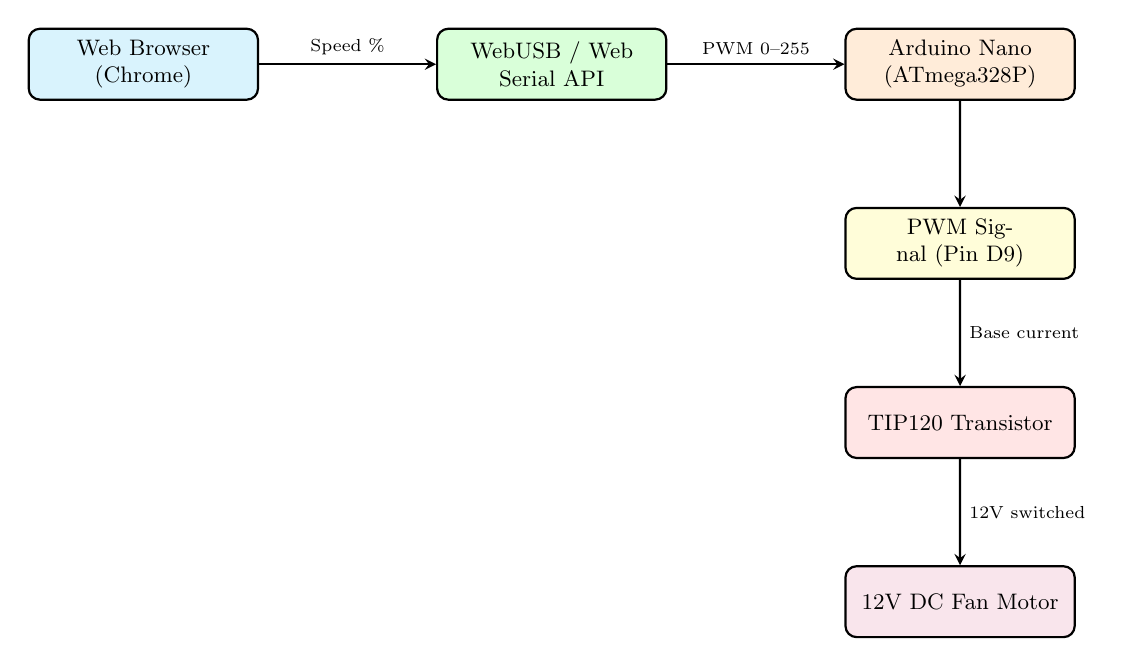
\begin{tikzpicture}[node distance=1.8cm, scale=0.9, transform shape,
    block/.style={rectangle, rounded corners, draw, thick, fill=blue!10, minimum width=3cm, minimum height=1cm, text centered, text width=3cm, font=\small},
    arr/.style={thick, ->, >=stealth}
]

\node[block, fill=cyan!15] (browser) {Web Browser (Chrome)};
\node[block, fill=green!15, right=2.5cm of browser] (usb) {WebUSB / Web Serial API};
\node[block, fill=orange!15, right=2.5cm of usb] (arduino) {Arduino Nano (ATmega328P)};
\node[block, fill=yellow!15, below=1.5cm of arduino] (pwm) {PWM Signal (Pin D9)};
\node[block, fill=red!10, below=1.5cm of pwm] (tip) {TIP120 Transistor};
\node[block, fill=purple!10, below=1.5cm of tip] (fan) {12V DC Fan Motor};

\draw[arr] (browser) -- node[above, font=\scriptsize] {Speed \%} (usb);
\draw[arr] (usb) -- node[above, font=\scriptsize] {PWM 0--255} (arduino);
\draw[arr] (arduino) -- (pwm);
\draw[arr] (pwm) -- node[right, font=\scriptsize] {Base current} (tip);
\draw[arr] (tip) -- node[right, font=\scriptsize] {12V switched} (fan);

\end{tikzpicture}
\caption{End-to-End Communication and Control Flow}
\label{fig:commflow}
\end{figure}

\newpage

% ===== SECTION 5: ARDUINO CODE =====
\section{Arduino Firmware (Source Code)}

The following firmware is uploaded to the Arduino Nano using the Arduino IDE. It listens for PWM values (0--255) sent via the serial port from the web browser and applies them to the fan motor using the \texttt{analogWrite()} function.

\subsection{Complete Source Code}

\begin{lstlisting}[style=arduinoStyle, caption={SmartBreeze -- Arduino Nano Firmware}, label={lst:arduino}]
// ============================================
// SmartBreeze Controller
// Target: Arduino Nano (ATmega328P)
// Author: Yogesh MN
// ============================================

const int fanPin = 9;       // PWM output pin (D9)
int currentSpeed = 0;       // Current fan speed (0-255)
String inputBuffer = "";    // Serial input buffer

void setup() {
  Serial.begin(9600);       // Initialize serial at 9600 baud
  pinMode(fanPin, OUTPUT);  // Set D9 as output
  analogWrite(fanPin, 0);   // Ensure fan starts OFF
}

void loop() {
  // Process incoming serial data character by character
  while (Serial.available() > 0) {
    char c = Serial.read();
    
    if (c == '\n') {
      // Newline received: parse the complete number
      int newSpeed = inputBuffer.toInt();
      
      // Validate range: 0 to 255
      if (inputBuffer.length() > 0 
          && newSpeed >= 0 
          && newSpeed <= 255) {
        currentSpeed = newSpeed;
        analogWrite(fanPin, currentSpeed);
      }
      
      // Clear buffer for next command
      inputBuffer = "";
    } 
    else if (c >= '0' && c <= '9') {
      // Accumulate numeric digits only
      inputBuffer += c;
    }
  }
  
  // Small delay to prevent CPU overuse
  delay(10);
}
\end{lstlisting}

\subsection{Code Explanation}

\begin{enumerate}
    \item \textbf{Initialization (setup):} The serial port is opened at 9600 baud, matching the web application's configured baud rate. Pin D9 is set as an output and initialized to 0 (fan off).
    
    \item \textbf{Character-by-Character Parsing:} Unlike \texttt{Serial.parseInt()} which has a blocking timeout that resets the fan to zero, this approach reads individual characters and accumulates them in a buffer. This ensures the fan \textbf{never stops unexpectedly} due to a communication timeout.
    
    \item \textbf{Newline Delimiter:} The web application sends each PWM value followed by a newline character (\textbackslash n). When the Arduino detects this delimiter, it knows a complete number has been received and safely parses it.
    
    \item \textbf{Range Validation:} The received value is checked to ensure it falls within the valid PWM range (0--255) before being applied to the fan output pin.
    
    \item \textbf{Persistent Speed:} The \texttt{currentSpeed} variable retains the last valid speed value. If no new serial data arrives, the fan continues running at the last commanded speed --- a critical design decision for continuous operation.
\end{enumerate}

\newpage

% ===== SECTION 6: WEB COMMUNICATION PROTOCOL =====
\section{Web Communication Protocol}

\subsection{Dual-Mode Architecture}
The web application implements a smart device-detection mechanism to ensure seamless connectivity across both desktop and mobile platforms:

\begin{table}[H]
\centering
\renewcommand{\arraystretch}{1.4}
\begin{tabular}{|>{\raggedright}p{3cm}|>{\raggedright}p{3.5cm}|>{\raggedright\arraybackslash}p{6cm}|}
\hline
\textbf{Platform} & \textbf{API Used} & \textbf{Reason} \\
\hline
Desktop (Windows, macOS, Linux) & Web Serial API & OS-level serial drivers provide native access. WebUSB is blocked by OS drivers. \\
\hline
Mobile (Android) & WebUSB API with FTDI Protocol & Android Chrome lacks full Web Serial support. WebUSB allows direct USB device communication. \\
\hline
\end{tabular}
\caption{Platform-Specific Communication Strategy}
\label{tab:protocol}
\end{table}

\subsection{FTDI Protocol Details (Mobile WebUSB)}
When connecting via WebUSB on Android, the application manually initializes the FTDI (Future Technology Devices International) USB-to-Serial converter chip present on the Arduino Nano using the following vendor-specific USB control transfers:

\begin{enumerate}
    \item \textbf{Device Reset:} Request \texttt{0x00} --- Resets the FTDI chip to a known state.
    \item \textbf{Baud Rate Configuration:} Request \texttt{0x03}, Value \texttt{0x4138} --- Sets communication speed to 9600 baud.
    \item \textbf{Data Format:} Request \texttt{0x04}, Value \texttt{0x0008} --- Configures 8 data bits, no parity, 1 stop bit (8N1).
    \item \textbf{Flow Control:} Request \texttt{0x02}, Value \texttt{0x0000} --- Disables hardware flow control.
\end{enumerate}

\subsection{Data Format}
Each speed command sent from the browser to the Arduino follows this format:
\begin{center}
\texttt{<PWM\_VALUE>\textbackslash n}
\end{center}
Where \texttt{PWM\_VALUE} is an integer between 0 and 255, and \texttt{\textbackslash n} is the newline delimiter. A keepalive signal is transmitted every 5 seconds to maintain connection integrity.

\newpage

% ===== SECTION 7: SAFETY =====
\section{Safety Considerations}

\begin{enumerate}
    \item \textbf{Flyback Diode Protection:} The 1N4007 diode across the fan terminals absorbs reverse voltage spikes generated when the motor's magnetic field collapses during PWM switching, preventing damage to the TIP120 transistor.
    
    \item \textbf{Current Limiting Resistor:} The 1K$\Omega$ resistor prevents excessive current draw from the Arduino's GPIO pin, which is rated for a maximum of 20mA.
    
    \item \textbf{Separate Power Rails:} The 12V fan power supply is kept separate from the Arduino's 5V logic supply. Only the ground is shared, preventing high-voltage feedback into the microcontroller.
    
    \item \textbf{Auto-Shutdown on Disconnect:} The web application sends a PWM value of 0 to the Arduino via the \texttt{beforeunload} browser event when the user closes the web page, ensuring the physical fan stops safely.
    
    \item \textbf{Thermal Considerations:} The TIP120 transistor may become slightly warm during extended operation. For the current application (small 12V fan drawing less than 300mA), no heatsink is required. The operating temperature remains well within safe limits.
\end{enumerate}

% ===== SECTION 8: REFERENCES =====
\section{References}
\begin{enumerate}
    \item Arduino Nano Documentation. Arduino.cc. Available: \url{https://docs.arduino.cc/hardware/nano/}
    \item TIP120 Darlington Transistor Datasheet. ON Semiconductor. Available: \url{https://www.onsemi.com/pdf/datasheet/tip120-d.pdf}
    \item WebUSB API Specification. W3C. Available: \url{https://wicg.github.io/webusb/}
    \item Web Serial API. W3C WICG. Available: \url{https://wicg.github.io/serial/}
    \item FTDI FT232R USB UART IC Datasheet. FTDI Ltd. Available: \url{https://ftdichip.com/products/ft232rl/}
    \item Open-Meteo Free Weather API. Available: \url{https://open-meteo.com/}
    \item Leaflet.js Interactive Maps. Vladimir Agafonkin. Available: \url{https://leafletjs.com/}
\end{enumerate}

\end{document}
